%\documentclass[letterpaper, twocolumn, 10pt]{article}
%\documentclass{acm_proc_article-sp}
\documentclass{sig-alternate}
\usepackage[hyphens]{url}
\usepackage[usenames,dvipsnames]{color}
\usepackage{comment}
\usepackage{float}
\usepackage{lipsum}
\usepackage{pifont} %used for tickmark and crosses.
% \usepackage[english]{babel}
\usepackage{array}
\usepackage{multirow}
\usepackage{amssymb}
%\usepackage{amsthm}
\usepackage{amsmath}
\usepackage[normalem]{ulem}
\usepackage{xspace}
\usepackage{datetime}

% To support subfigures
%\usepackage{caption}
%\usepackage{subcaption}

% \usepackage{graphicx}

%%%%%%%%%% verbatim related
\usepackage{fancyvrb}
%\usepackage{fixltx2e}
\fvset{framesep=2mm,fontsize=\scriptsize,framerule=.1mm,numbersep=1mm,commandchars=\\\{\}}
\usepackage{listings}
% \usepackage{tgcursor}

%%%%%%%%%%%%%%%%%%%% pseudocode-related stuff
\usepackage[usenames,dvipsnames]{xcolor}
\newcommand{\codecomment}[1]{\textcolor[rgb]{0.133,0.445,0.133}{#1}}
\usepackage{algorithm}
\usepackage[noend]{algpseudocode}
% \usepackage{algorithmic}
\newfloat{algorithm}{t}{lop}
% change indentation!!
\renewcommand\algorithmicindent{1em}
%\newcommand{\INDSTATE}[1][1]{\State\hspace{#1\algorithmicindent}}
% \newcommand{\INDSTATE}[1][1]{\State\hspace{2em}}
%%%%%%%%%%%%%%%%%%%%

% float control
\renewcommand{\topfraction}{0.9}

\widowpenalty=10000
\clubpenalty=10000

% \usepackage[small,compact]{titlesec}

% \usepackage{savetrees}

%%%%%%%%%%%%%%%%%%%%

\newtheorem{mydef}{Definition}
\newtheorem{theorem}{Theorem}[section]
\newsavebox{\verbbox}
% \usepackage[stable]{footmisc}

\newif\ifrev

\hyphenation{WEB-rick}

%%%%%%%%%%%%%%%%%%
\usepackage{hyperref}


%%%%%%%%%%%%%%%%%%
% COMMENT OUT NEXT LINE TO HIDE TODOs
\revtrue
%%%%%%%%%%%%%%%%%%

\ifrev
  \newcommand{\todo}[1]{{\color{red} [TODO: #1]}}
\else
  \newcommand{\todo}[1]{}
\fi

\newcommand{\eat}[1]{}
\newcolumntype{m}[1]{>{\centering\arraybackslash\hspace{0pt}}p{#1}}
\renewcommand\arraystretch{1.5} % so exponents fit inside a table
\newcommand{\bigO}[1]{\ensuremath{\operatorname{O}\bigl(#1\bigr)}}
\newcommand\vit[1]{\textit{#1}}
% \renewcommand{\theFancyVerbLine}{\textsuperscript{\arabic{FancyVerbLine}}}
% big-O notation/symbol

\newcommand{\sysname}{DockerSecrets\xspace}


\newenvironment{myquote}{\list{}{\leftmargin=0in\rightmargin=0in}\item[]}{
\endlist}

\makeatletter
\newcommand\xleftrightarrow[2][]{%
  \ext@arrow 9999{\longleftrightarrowfill@}{#1}{#2}}
\newcommand\longleftrightarrowfill@{%
  \arrowfill@\leftarrow\relbar\rightarrow}
\makeatother

\renewcommand{\labelenumi}{\roman{enumi}}
\newcounter{mycounter}
\newenvironment{noindlist}
 {\begin{list}{\textit{\arabic{mycounter})}~}{\usecounter{mycounter}
\labelsep=0em
\labelwidth=0em \leftmargin=0em \itemindent=1em \itemsep=-0.2em }}
 {\end{list}}

\newcommand{\squishlist}{%
   \begin{list}{$\bullet$}
    { \setlength{\itemsep}{0pt}      \setlength{\parsep}{3pt}
      \setlength{\topsep}{3pt}       \setlength{\partopsep}{0pt}
      \setlength{\leftmargin}{1.5em} \setlength{\labelwidth}{1em}
      \setlength{\labelsep}{0.5em} } }

\newcommand{\squishend}{%
    \end{list}  }

\newcommand{\tickmark}{\ding{51}}
\newcommand{\xmark}{\ding{55}}

\newcommand*\samethanks[1][\value{footnote}]{\footnotemark[#1]}


\usepackage{ifthen}
\usepackage[normalem]{ulem} % for \sout
\usepackage{xcolor}
\let\lneq\undefined  % removes amssymb conflict with some packages
\usepackage{amssymb}
\newcommand{\ra}{$\rightarrow$}
\newboolean{showedits}
\setboolean{showedits}{true} % toggle to show or hide edits
\ifthenelse{\boolean{showedits}}
{
	\newcommand{\ugh}[1]{\textcolor{red}{\uwave{#1}}} % please rephrase
	\newcommand{\ins}[1]{\textcolor{blue}{\uline{#1}}} % please insert
	\newcommand{\del}[1]{\textcolor{red}{\sout{#1}}} % please delete
	\newcommand{\chg}[2]{\textcolor{red}{\sout{#1}}{\ra}\textcolor{blue}{\uline{#2}}} % please change
}{
	\newcommand{\ugh}[1]{#1} % please rephrase
	\newcommand{\ins}[1]{#1} % please insert
	\newcommand{\del}[1]{} % please delete
	\newcommand{\chg}[2]{#2}
}

\newboolean{showcomments}
%\setboolean{showcomments}{true}
\setboolean{showcomments}{true}
\newcommand{\id}[1]{$-$Id: scgPaper.tex 32478 2010-04-29 09:11:32Z oscar $-$}
\newcommand{\yellowbox}[1]{\fcolorbox{gray}{yellow}{\bfseries\sffamily\scriptsize#1}}
\newcommand{\triangles}[1]{{\sf\small$\blacktriangleright$\textit{#1}$\blacktriangleleft$}}
\ifthenelse{\boolean{showcomments}}
%{\newcommand{\nb}[2]{{\yellowbox{#1}\triangles{#2}}}
{\newcommand{\nbc}[3]{
 {\colorbox{#3}{\bfseries\sffamily\scriptsize\textcolor{white}{#1}}}
 {\textcolor{#3}{\sf\small$\blacktriangleright$\textit{#2}$\blacktriangleleft$}}}
 \newcommand{\version}{\emph{\scriptsize\id}}}
{\newcommand{\nbc}[3]{}
 \renewcommand{\ugh}[1]{#1} % please rephrase
 \renewcommand{\ins}[1]{#1} % please insert
 \renewcommand{\del}[1]{} % please delete
 \renewcommand{\chg}[2]{#2} % please change
 \newcommand{\version}{}}
\newcommand{\nb}[2]{\nbc{#1}{#2}{orange}}

\definecolor{jccolor}{rgb}{0.2,0.4,0.6}
\definecolor{clcolour}{rgb}{0.5,0.7,0.9}
\newcommand\cappos[1]{\nbc{JC}{#1}{jccolor}}
\newcommand\diogo[1]{\nbc{DM}{#1}{clcolor}}
\usepackage{wasysym}


\begin{document}

\numberofauthors{2}
%\date{}

\title{\sysname: How To Keep a Distributed Secret}


% enable this to de-anonymize!
%\newcommand{\showurlx}{{\url{https://whatever_the_url.is}}}
\newcommand{\showurlx}{[redacted]}

\author{
Diogo, Riyaz, Ying Li, ?Laurens Van Houtven?, ?Nathan?, ..., Justin
%\IEEEauthorblockN{Justin Cappos}\\
%New York University\\
%jcappos@nyu.edu
%\and
%Author list goes here.
% copy the following lines to add more authors
% \and
% {\rm Name}\\
%Name Institution
}

\maketitle

\begin{abstract}

Secrets, such as database passwords and private keys are 
a key part of security systems.  Unfortunately, secrets are hard to securely 
distribute, rotate, and revoke, especially without changing existing software.

To address these issues, a technique called \sysname has been developed.
\sysname automatically provisions containers with secrets without
requiring the use of environment variables.  It also ensures that applications
obtains a secret in a natural way, reading a file from disk, instead of 
requiring application modification to call a custom API or to possess 
specialized hardware (e.g., SGX).  Additionally, 
Docker secrets are securely distributed and are never stored or transmitted 
in an unencrypted form.  Information stored in Docker secrets can be changed 
and revoked automatically, which enables better dev ops security practices, 
such as hourly TLS key rotation.  The deployment of Docker secrets has been
in production since Docker 1.13, and is running in ?millions? of containers.


\end{abstract}

\section{Introduction}
\label{SEC:introduction}

\cappos{I think there is some quote about it being hard to keep secrets.}

Secrets are hard to keep, especially when they are shared.  Computer systems
are not immmune to this phenomenon.  
One of the most challenging problems
involves the effective provisioning of secrets.  Common secrets of this
sort are TLS keys and certificates, passwords, internal server names, and SSH 
keys \cappos{possible cites}.  

Unfortunately, provisioning secrets securely is hard, leading to unintended
disclosure of sensitive information.  Fairly commonly, secrets are 
accidentally checked into version control systems, emitted in logs, or 
...   Furthermore, due to the difficulty of secure provisioning, secrets
are also commonly shared between test and production environments, leading
to both accidents and malicious behavior.
\cappos{mention you can give Travis secrets in some way.  However, it leaks 
those secrets by printing them in log files (unencrypted).}

\cappos{Perhaps motivate how containers / service computing is increasing 
the number of small, distributed items in a server here.}

The reason why it is hard to securely provision
secrets is due to four factors.  
\begin{itemize}
\item {\bf API.} First, the mechanisms used to provide
secrets, such as environment variables or custom APIs, require substantial
vigilence from dev ops personnel to avoid being leaked~\cappos{cite 
Perforce was storing FreeBSD core
dumps.  Those core dumps had environment variables (w/ secrets) that were
available publicly accidentally.}   
\item {\bf persistance.} Second, secrets must be stored
\emph{somewhere} to survive power cycling.  There needs to be a way to 
securely persist secrets so that an attacker cannot gain access.
\item {\bf distribution.} Third, the secrets must be securely distributed
to an array of different container or service instances.  Ensuring that
each recipient is authorized to receive a secret is paramount, as is
following the principle of least privilege to provide only the needed
secrets.
\item {\bf rotation.} Finally, despite the best effort of systems
implementers, history has shown that security bugs arise in even
the best tested code.  It is important to have a secure, responsive, and
usable mechanism for revoking and rotating secrets.  
\end{itemize}


%Brief:
%dm-verify / secure dep / image resolution.  Just want to be sure we have 
%some way to explain how we know who to give the secret to in the first place
%and what information to share.
%Run system services in containers
%
%Core: 
%+ Secure container platform / swarm setup (Swarmkit / Notary)
%+ Root of trust rotation
%+ Rotate keys / certs in and out of the hands of third parties
%+ secure node introduction.  How infrakit gets keys there in the first place.
%(Infrakit / Swarmkit)
%+ reverse uptime to bound liveness of nodes.  (Infrakit)
%(Can you enforce this on a compromised system?)  
%+ Mutual TLS between nodes. (Is this Swarmkit???)




In this paper, we present \sysname, a novel technique for addressing
the secret distribution problem in distributed systems.  While
\sysname is part of a broader ecosystem, it primarily extends three key 
components (SwarmKit, InfraKit, and Notary) to distribute, persist, and 
rotate secrets.  Containers are securely validated for both correctness and
freshness.  Validation is done prior to secret information being shared with 
them through the use of cryptographic node
identities.  Much like the rights field and check bits concepts common
to many capability-based access control systems, these identities embed
node roles, root CA information, and proof of the right to join the swarm
in X509 certificates.  

Shared secrets are also used to transparently set up secure intra-service 
and inter-service communications channels.  All communication between
services \cappos{even on the same physical server?} is done using mutual
TLS authentication.  This prevents man-in-the-middle attackers from
intercepting communications between services or impersonating a service
in communications.  

\sysname is designed to minimize the impact of a successful attack, with
key rotation a central part of the design.  All keys can be transparently
rotated without operator or service intervention \cappos{???}.  
This includes rotating the root of trust inside of a set of containers,
possibly migrating trust to and from third party CAs as desired.   The
ability to quickly and seamlessly rotate keys  means that keys may be 
replaced often --- limiting an attacker's ability to cause damage after 
a successful breach.  In fact, in production many users of \sysname
use this mechanism to automatically rotate their secrets every hour.


To ensure that images are correct and fresh, this work introduces the 
concept of \emph{reverse uptime}.  Reverse uptime provides a duration which
a service is permitted to live.  Once this value reaches zero, the service
is automatically killed \cappos{How does this work?  Is the cryptographic
node identity also revoked?  As I understand it, these would be separate
mechanisms...}  This ensures that services constantly are installing fresh
images.  It also may have the side effect of reducing the amount of time an
attaker that compromises a service has to utilize that access.

Since \sysname is designed to be seamless to deploy, it is easy use 
in many 
\sysname has been deployed in production in Docker since 1.13, leading to 
use in millions of swarms.  This practical experience, uncovered several
non-obvious lessons from \sysname.  First, while \sysname does not have the 
same security guarantees as specialized designs (e.g., SGX, which requires
specialized hardware), the usability and seamless nature of \sysname makes it
possible to quickly deploy in many environments.    Second, ..., Finally, ...
As a result, \sysname has improved the security of millions of containers.


The primary contributions of this work are as follows:

\begin{itemize}

\item This work describes a series of novel techniques to enable secrets to
be securely shared between containers.  This includes techniques to
securely introduce nodes to each other, automatic provisioning of mutual
TLS connections (even for the application's connections), as well as reverse 
uptime and rotation of secrets to bound the impact of a compromise.

\item \sysname was designed based upon pragmatic decisions that maximize 
ease of deployment.  For example, \sysname maps in each secret
as though it is a file in the file system.  This means that applications
need not be modified to use \sysname.  

\item Careful engineering of \sysname demonstrates that security need not
come at the cost of performance.  \sysname adds only X\% overhead in 
bandwidth, a XXms container startup latency, and XXXX when rotating
secrets.


\end{itemize}




\section{Background}
\label{SEC:background}

\cappos{Introduce all of the components we need for this work.  I am not sure
yet whether there should be a large section talking about this here or
whether this should be in the architecture section.  Splitting either way
seems like it has reasonable pros and cons.}




\section{\sysname}
\label{SEC:architecture}

\cappos{this section is meant to describe the mechanisms / changes that were
made to docker to support \sysname.  So, one likely organization would be
to discuss each of the components (infrakit, swarmkit, notary) in some detail
while emphasizing the mechanisms that were added.  I've started the section
with an example to get it started}

There are three critical components that have been altered that enable
\sysname (Figure~XXX\cappos{need to add}).  First, infrakit is the component 
of Docker which handles container
instantiation and XXX on a local system.  Infrakit was modified by changing
YYY to enable ZZZ.   Swarmkit enables the instantatiation and management of 
groups of containers by XXX.  ...

\subsection{Infrakit}

\cappos{describe purpose and concepts about how this is designed.  Try to 
avoid talking too much about how it is actually used at this point.  To 
think of a car analogy, you don't want a user's manual here, you want the
mechanics guide / tech specs for making the components.}


\subsection{Swarmkit}
Swarmkit handles mutual TLS, ...


\subsection{Notary}
Notary enables key expiry, trust anchoring, etc...

\cappos{Content from:
\url{https://docs.docker.com/engine/security/trust/content_trust/}}



When transferring data among networked systems, trust is a central concern.
In particular, when communicating over an untrusted medium such as the
internet, it is critical to ensure the integrity and the publisher of all
the data a system operates on. You use Docker Engine to push and pull
images (data) to a public or private registry. Content trust gives you the
ability to verify both the integrity and the publisher of all the data
received from a registry over any channel.

\subsubsection{Understanding trust in Docker}
Content trust allows operations with a remote Docker registry to enforce
client-side signing and verification of image tags. Content trust provides
the ability to use digital signatures for data sent to and received from
remote Docker registries. These signatures allow client-side verification
of the integrity and publisher of specific image tags.

Currently, content trust is disabled by default. To enable it, set the
{\tt DOCKER\_CONTENT\_TRUST} environment variable to 1. Refer to the environment
variables and Notary configuration for the docker client for more options.

Once content trust is enabled, image publishers can sign their images.
Image consumers can ensure that the images they use are signed. Publishers
and consumers can be individuals alone or in organizations. Docker’s
content trust supports users and automated processes such as builds.

\subsubsection{Image tags and content trust}
An individual image record has the following identifier:

\begin{quote}
[REGISTRY\_HOST[:REGISTRY\_PORT]/]REPOSITORY[:TAG]
\end{quote}

A particular image REPOSITORY can have multiple tags. For example, latest
and 3.1.2 are both tags on the mongo image. An image publisher can build an
image and tag combination many times changing the image with each build.

Content trust is associated with the TAG portion of an image. Each image
repository has a set of keys that image publishers use to sign an image
tag. Image publishers have discretion on which tags they sign.

An image repository can contain an image with one tag that is signed and
another tag that is not (Figure~\ref{fig-notary-tag-signing}). For example, 
consider the Mongo image repository.
The latest tag could be unsigned while the 3.1.6 tag could be signed. It is
the responsibility of the image publisher to decide if an image tag is
signed or not. In this representation, some image tags are signed, others
are not:

\begin{figure}[t]
  \center{}
  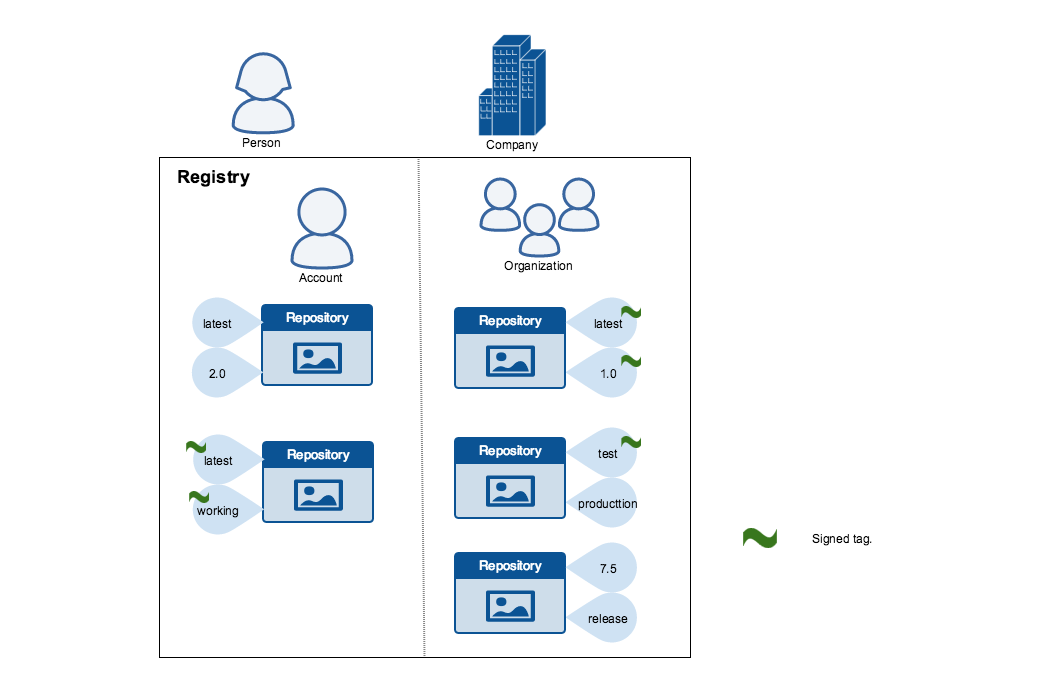
\includegraphics[width=.5\textwidth]{images/notary_tag_signing.png}
  \caption{Tag signing in Notary.
  \label{fig-notary-tag-signing} }
\end{figure}

Publishers can choose to sign a specific tag or not. As a result, the
content of an unsigned tag and that of a signed tag with the same name may
not match. For example, a publisher can push a tagged image
someimage:latest and sign it. Later, the same publisher can push an
unsigned someimage:latest image. This second push replaces the last
unsigned tag latest but does not affect the signed latest version. The
ability to choose which tags they can sign, allows publishers to iterate
over the unsigned version of an image before officially signing it.

Image consumers can enable content trust to ensure that images they use
were signed. If a consumer enables content trust, they can only pull, run,
or build with trusted images. Enabling content trust is like wearing a pair
of rose-colored glasses. Consumers “see” only signed image tags and the
less desirable, unsigned image tags are “invisible” to them.

\begin{figure}[t]
  \center{}
  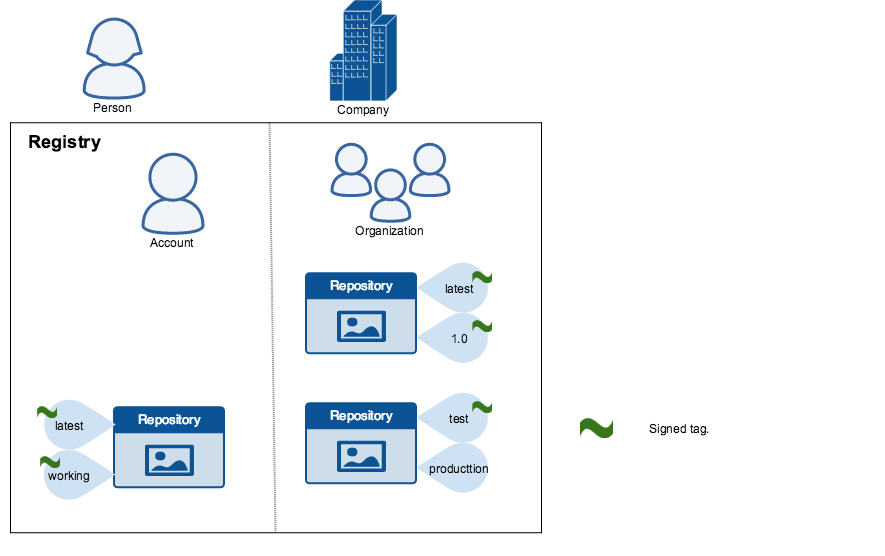
\includegraphics[width=.5\textwidth]{images/notary_trust_view.png}
  \caption{
This figure depicts the various signing keys and their
relationships.  \cappos{Where is this figure used in the text?}
  \label{fig-notary-trust-view} }
\end{figure}

To the consumer who has not enabled content trust, nothing about how they
work with Docker images changes. Every image is visible regardless of
whether it is signed or not.

\subsubsection{Content trust operations and keys}
When content trust is enabled, docker CLI commands that operate on tagged
images must either have content signatures or explicit content hashes. The
commands that operate with content trust are:

push
build
create
pull
run
For example, with content trust enabled a docker pull someimage:latest only
succeeds if someimage:latest is signed. However, an operation with an
explicit content hash always succeeds as long as the hash exists:

\begin{quote}
\$ docker pull
someimage@sha256:d149ab53f8718e987c3a3024bb8aa0e2caadf6c0328f1d9d850b2a2a67f2819a
\end{quote}

Trust for an image tag is managed through the use of signing keys. A key
set is created when an operation using content trust is first invoked. A
key set consists of the following classes of keys:

\begin{itemize}
\item an offline key that is the root of content trust for an image tag
repository or tagging keys that sign tags
\item server-managed keys such as the timestamp key, which provides freshness
security guarantees for your repository
\end{itemize}

\begin{figure}[t]
  \center{}
  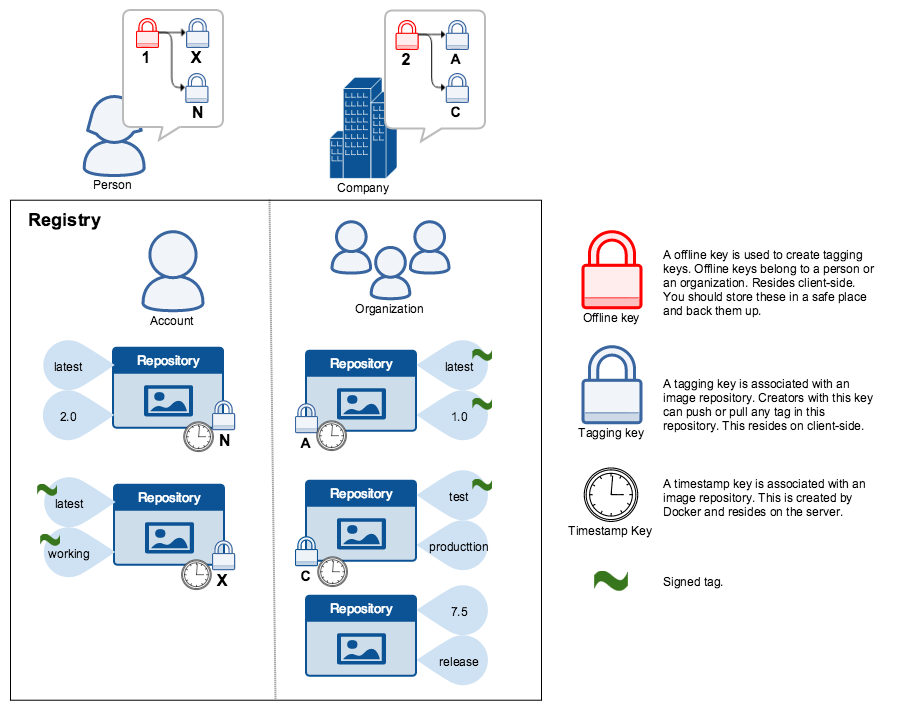
\includegraphics[width=.5\textwidth]{images/notary_trust_components.png}
  \caption{
This figure depicts the various signing keys and their
relationships.
  \label{fig-notary-components} }
\end{figure}

WARNING: Loss of the root key is very difficult to recover from. Correcting
this loss requires intervention from Docker Support to reset the repository
state. This loss also requires manual intervention from every consumer that
used a signed tag from this repository prior to the loss.
You should backup the root key somewhere safe. Given that it is only
required to create new repositories, it is a good idea to store it offline
in hardware. For details on securing, and backing up your keys, make sure
you read how to manage keys for content trust.

\subsubsection{Survey of typical content trust operations}
This section surveys the typical trusted operations users perform with
Docker images. Specifically, we will be going through the following steps
to help us exercise these various trusted operations:

Build and push an unsigned image
Pull an unsigned image
Build and push a signed image
Pull the signed image pushed above
Pull unsigned image pushed above
Enable and disable content trust per-shell or per-invocation
In a shell, you can enable content trust by setting the
{\tt DOCKER\_CONTENT\_TRUST} environment variable. Enabling per-shell is useful
because you can have one shell configured for trusted operations and
another terminal shell for untrusted operations. You can also add this
declaration to your shell profile to have it turned on always by default.

To enable content trust in a bash shell enter the following command:

\begin{quote}
export DOCKER\_CONTENT\_TRUST=1
\end{quote}

Once set, each of the “tag” operations requires a key for a trusted tag.

In an environment where {\tt DOCKER\_CONTENT\_TRUST} is set, you can use the
--disable-content-trust flag to run individual operations on tagged images
without content trust on an as-needed basis.

Consider the following Dockerfile that uses an untrusted base image:

\begin{quote}
\$  cat Dockerfile
FROM docker/trusttest:latest
RUN echo
\end{quote}

In order to build a container successfully using this Dockerfile, one can
do:

\begin{quote}
\$  docker build --disable-content-trust -t <username>/nottrusttest:latest .
Sending build context to Docker daemon 42.84 MB
...
Successfully built f21b872447dc
\end{quote}

The same is true for all the other commands, such as pull and push:

\begin{quote}
\$  docker pull --disable-content-trust docker/trusttest:latest
...
\$  docker push --disable-content-trust <username>/nottrusttest:latest
...
\end{quote}

To invoke a command with content trust enabled regardless of whether or how
the {\tt DOCKER\_CONTENT\_TRUST} variable is set:

\begin{quote}
\$  docker build --disable-content-trust=false -t
<username>/trusttest:testing .
\end{quote}

All of the trusted operations support the --disable-content-trust flag.

\subsubsection{Push trusted content}
To create signed content for a specific image tag, simply enable content
trust and push a tagged image. If this is the first time you have pushed an
image using content trust on your system, the session looks like this:

\begin{quote}
\$ docker push <username>/trusttest:testing
The push refers to a repository [docker.io/<username>/trusttest] (len: 1)
9a61b6b1315e: Image already exists
902b87aaaec9: Image already exists
latest: digest:
sha256:d02adacee0ac7a5be140adb94fa1dae64f4e71a68696e7f8e7cbf9db8dd49418
size: 3220
Signing and pushing trust metadata
You are about to create a new root signing key passphrase. This passphrase
will be used to protect the most sensitive key in your signing system.
Please
choose a long, complex passphrase and be careful to keep the password and
the
key file itself secure and backed up. It is highly recommended that you use
a
password manager to generate the passphrase and keep it safe. There will be
no
way to recover this key. You can find the key in your config directory.
Enter passphrase for new root key with id a1d96fb:
Repeat passphrase for new root key with id a1d96fb:
Enter passphrase for new repository key with id
docker.io/<username>/trusttest (3a932f1):
Repeat passphrase for new repository key with id
docker.io/<username>/trusttest (3a932f1):
Finished initializing "docker.io/<username>/trusttest"
\end{quote}

When you push your first tagged image with content trust enabled, the
docker client recognizes this is your first push and:

alerts you that it will create a new root key
requests a passphrase for the root key
generates a root key in the ~/.docker/trust directory
requests a passphrase for the repository key
generates a repository key in the ~/.docker/trust directory
The passphrase you chose for both the root key and your repository key-pair
should be randomly generated and stored in a password manager.

NOTE: If you omit the testing tag, content trust is skipped. This is true
even if content trust is enabled and even if this is your first push.
\begin{quote}
\$ docker push <username>/trusttest
The push refers to a repository [docker.io/<username>/trusttest] (len: 1)
9a61b6b1315e: Image successfully pushed
902b87aaaec9: Image successfully pushed
latest: digest:
sha256:a9a9c4402604b703bed1c847f6d85faac97686e48c579bd9c3b0fa6694a398fc
size: 3220
No tag specified, skipping trust metadata push
\end{quote}

It is skipped because as the message states, you did not supply an image
TAG value. In Docker content trust, signatures are associated with tags.

Once you have a root key on your system, subsequent images repositories you
create can use that same root key:

\begin{quote}
\$ docker push docker.io/<username>/otherimage:latest
The push refers to a repository [docker.io/<username>/otherimage] (len: 1)
a9539b34a6ab: Image successfully pushed
b3dbab3810fc: Image successfully pushed
latest: digest:
sha256:d2ba1e603661a59940bfad7072eba698b79a8b20ccbb4e3bfb6f9e367ea43939
size: 3346
Signing and pushing trust metadata
Enter key passphrase for root key with id a1d96fb:
Enter passphrase for new repository key with id
docker.io/<username>/otherimage (bb045e3):
Repeat passphrase for new repository key with id
docker.io/<username>/otherimage (bb045e3):
Finished initializing "docker.io/<username>/otherimage"
\end{quote}

The new image has its own repository key and timestamp key. The latest tag
is signed with both of these.

\subsubsection{Pull image content}
A common way to consume an image is to pull it. With content trust enabled,
the Docker client only allows docker pull to retrieve signed images. Let’s
try to pull the image you signed and pushed earlier:

\begin{quote}
\$  docker pull <username>/trusttest:testing
Pull (1 of 1): <username>/trusttest:testing@sha256:d149ab53f871
...
Tagging <username>/trusttest@sha256:d149ab53f871 as
docker/trusttest:testing
\end{quote}

In the following example, the command does not specify a tag, so the system
uses the latest tag by default again and the docker/trusttest:latest tag is
not signed.

\begin{quote}
\$ docker pull docker/trusttest
Using default tag: latest
no trust data available
\end{quote}

Because the tag docker/trusttest:latest is not trusted, the pull fails.

\cappos{the notary text was too much like running examples.  It needs to focus
on the design at a higher level.}

\section{Examples Using \sysname}
\label{SEC:examples}

\cappos{This section is end-to-end examples that show all of the pieces coming
together.  Here, the paper discusses how to accomplish high level tasks
(key rotation, etc.) using the pieces from the prior section.}




\subsection{Introducing Docker Secrets Management}
\cappos{Taken from:
\url{https://blog.docker.com/2017/02/docker-secrets-management/}}

\cappos{This text needs to talk about how Notary, Swarmkit, Infrakit, etc.
work together to make this happen.}

We fundamentally believe that apps are safer if there is a standardized
interface for accessing secrets. Any good solution will also have to follow
security best practices, such as encrypting secrets while in transit;
encrypting secrets at rest; preventing secrets from unintentionally leaking
when consumed by the final application; and strictly adhere to the
principle of least-privilege, where an application only has access to the
secrets that it needs—no more, no less.

By integrating secrets into Docker orchestration, we are able to deliver a
solution for the secrets management problem that follows these exact
principles, as is shown in Figure~\ref{fig-swarm-arch}..

\begin{figure}[t]
  \center{}
  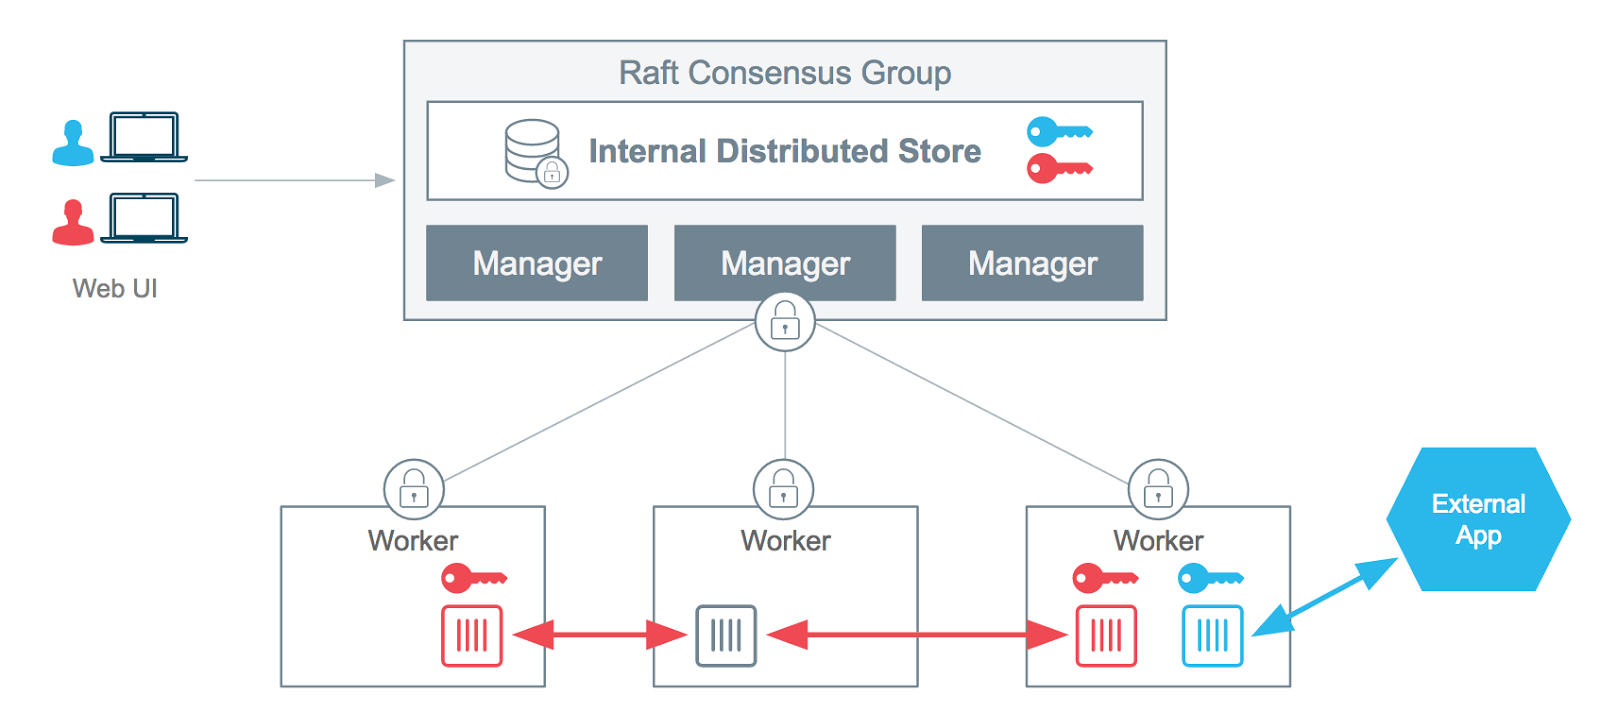
\includegraphics[width=.5\textwidth]{images/swarm_architecture.png}
  \caption{A high-level view of how the Docker swarm
mode architecture is applied to securely deliver a new type of object to
our containers: a secret object.
  \label{fig-swarm-arch} }
\end{figure}




In Docker, a secret is any blob of data, such as a password, SSH private
key, TLS Certificate, or any other piece of data that is sensitive in
nature. When you add a secret to the swarm (by running docker secret
create), Docker sends the secret over to the swarm manager over a mutually
authenticated TLS connection, making use of the built-in Certificate
Authority that gets automatically created when bootstrapping a new swarm.

 
\begin{quote}
\$ echo "This is a secret" | docker secret create my\_secret\_data -
\end{quote}
 

Once the secret reaches a manager node, it gets saved to the internal Raft
store, which uses NACL’s Salsa20Poly1305 with a 256-bit key to ensure no
data is ever written to disk unencrypted. Writing to the internal store
gives secrets the same high availability guarantees that the the rest of
the swarm management data gets.

When a swarm manager starts up, the encrypted Raft logs containing the
secrets is decrypted using a data encryption key that is unique per-node.
This key, and the node’s TLS credentials used to communicate with the rest
of the cluster, can be encrypted with a cluster-wide key encryption key,
called the unlock key, which is also propagated using Raft and will be
required on manager start.

When you grant a newly-created or running service access to a secret, one
of the manager nodes (only managers have access to all the stored secrets
stored) will send it over the already established TLS connection
exclusively to the nodes that will be running that specific service. This
means that nodes cannot request the secrets themselves, and will only gain
access to the secrets when provided to them by a manager – strictly for the
services that require them.

\begin{quote}
\$ docker service  create --name="redis" --secret="my\_secret\_data" redis:alpine
\end{quote}
 

The  unencrypted secret is mounted into the container in an in-memory
filesystem at /run/secrets/<secret\_name>.

\begin{quote}
\$ docker exec \$(docker ps --filter name=redis -q) ls -l /run/secrets
total 4
-r--r--r--    1 root     root            17 Dec 13 22:48 my\_secret\_data
\end{quote}
 

If a service gets deleted, or rescheduled somewhere else, the manager will
immediately notify all the nodes that no longer require access to that
secret to erase it from memory, and the node will no longer have any access
to that application secret.

\begin{quote}
\$ docker service update --secret-rm="my\_secret\_data" redis

\$ docker exec -it \$(docker ps --filter name=redis -q) cat /run/secrets/my\_secret\_data

cat: can't open '/run/secrets/my\_secret\_data': No such file or directory
\end{quote}


\bigskip
\cappos{This is pretty much similar text, but with different detail /
 emphasis.  Comes from:
\url{https://docs.docker.com/engine/swarm/secrets/\#about-secrets} }


In terms of Docker Swarm services, a secret is a blob of data, such as a
password, SSH private key, SSL certificate, or another piece of data that
should not be transmitted over a network or stored unencrypted in a
Dockerfile or in your application’s source code. In Docker 1.13 and higher,
you can use Docker secrets to centrally manage this data and securely
transmit it to only those containers that need access to it. Secrets are
encrypted during transit and at rest in a Docker swarm. A given secret is
only accessible to those services which have been granted explicit access
to it, and only while those service tasks are running.

You can use secrets to manage any sensitive data which a container needs at
runtime but you don’t want to store in the image or in source control, such
as:

\begin{itemize}
\item Usernames and passwords
\item TLS certificates and keys
\item SSH keys
\item Other important data such as the name of a database or internal server
\item Generic strings or binary content (up to 500 kb in size)
\end{itemize}

%Note: Docker secrets are only available to swarm services, not to
%standalone containers. To use this feature, consider adapting your
%container to run as a service with a scale of 1.

Another use case for using secrets is to provide a layer of abstraction
between the container and a set of credentials. Consider a scenario where
you have separate development, test, and production environments for your
application. Each of these environments can have different credentials,
stored in the development, test, and production swarms with the same secret
name. Your containers only need to know the name of the secret in order to
function in all three environments.

\subsubsection{How Docker manages secrets}
When you add a secret to the swarm, Docker sends the secret to the swarm
manager over a mutual TLS connection. The secret is stored in the Raft log,
which is encrypted. The entire Raft log is replicated across the other
managers, ensuring the same high availability guarantees for secrets as for
the rest of the swarm management data.

%Warning: Raft data is encrypted in Docker 1.13 and higher. If any of your
%Swarm managers run an earlier version, and one of those managers becomes
%the manager of the swarm, the secrets will be stored unencrypted in that
%node’s Raft logs. Before adding any secrets, update all of your manager
%nodes to Docker 1.13 to prevent secrets from being written to plain-text
%Raft logs.
When you grant a newly-created or running service access to a secret, the
decrypted secret is mounted into the container in an in-memory filesystem
at /run/secrets/<secret\_name>. You can update a service to grant it access
to additional secrets or revoke its access to a given secret at any time.

A node only has access to (encrypted) secrets if the node is a swarm
manager or if it is running service tasks which have been granted access to
the secret. When a container task stops running, the decrypted secrets
shared to it are unmounted from the in-memory filesystem for that container
and flushed from the node’s memory.

If a node loses connectivity to the swarm while it is running a task
container with access to a secret, the task container still has access to
its secrets, but cannot receive updates until the node reconnects to the
swarm.

You can add or inspect an individual secret at any time, or list all
secrets. You cannot remove a secret that a running service is using. See
Rotate a secret for a way to remove a secret without disrupting running
services.

In order to update or roll back secrets more easily, consider adding a
version number or date to the secret name. This is made easier by the
ability to control the mount point of the secret within a given container.

\subsubsection{Detailed example using secrets}

\cappos{Consider making an example that has enough interesting detail that
the reader gets all of the value from the three examples on:
\url{https://docs.docker.com/engine/swarm/secrets/\#examples}   This example
should be slightly more high level than it is currently.  It's too much of
a 'type this with me' guide and doesn't explain why or what is happening
enough..}

This simple example shows how secrets work in just a few commands. 
\begin{enumerate}
\item To add a secret to Docker, the user runs the {\tt docker 
secret create} command, as follows.   
\begin{quote}
\$ echo "This is a secret" | docker secret create my\_secret\_data -
\end{quote}

In this example, the command reads standard input because the last argument, 
which represents the file to read the secret from, is set to -.
\cappos{what's the point of this?  The secret ends up in your shell's
history this way?}


\item
Create a redis service and grant it access to the secret. By default, the
container can access the secret at /run/secrets/<secret\_name>, but you can
customize the file name on the container using the target option.

\begin{quote}
\$ docker service  create --name="redis" --secret="my\_secret\_data"
redis:alpine
\end{quote}

\item
Verify that the task is running without issues using docker service ps. If
everything is working, the output looks similar to this:

\begin{quote}
\$ docker service ps redis

ID            NAME     IMAGE         NODE              DESIRED STATE
CURRENT STATE          ERROR  PORTS
bkna6bpn8r1a  redis.1  redis:alpine  ip-172-31-46-109  Running
Running 8 seconds ago  
\end{quote}

If there were an error, and the task were failing and repeatedly
restarting, you would see something like this:

\begin{quote}
\$ docker service ps redis

NAME                      IMAGE         NODE  DESIRED STATE  CURRENT STATE
ERROR                      PORTS
redis.1.siftice35gla      redis:alpine  moby  Running        Running 4
seconds ago                             
 \_ redis.1.whum5b7gu13e  redis:alpine  moby  Shutdown       Failed 20
seconds ago      "task: non-zero exit (1)"  
 \_ redis.1.2s6yorvd9zow  redis:alpine  moby  Shutdown       Failed 56
seconds ago      "task: non-zero exit (1)"  
 \_ redis.1.ulfzrcyaf6pg  redis:alpine  moby  Shutdown       Failed about a
minute ago  "task: non-zero exit (1)"  
 \_ redis.1.wrny5v4xyps6  redis:alpine  moby  Shutdown       Failed 2
minutes ago       "task: non-zero exit (1)"
\end{quote}

\item
Get the ID of the redis service task container using docker ps , so that
you can use docker exec to connect to the container and read the contents
of the secret data file, which defaults to being readable by all and has
the same name as the name of the secret. The first command below
illustrates how to find the container ID, and the second and third commands
use shell completion to do this automatically.

\begin{quote}
\$ docker ps --filter name=redis -q

5cb1c2348a59

\$ docker exec \$(docker ps --filter name=redis -q) ls -l /run/secrets

total 4
-r--r--r--    1 root     root            17 Dec 13 22:48 my\_secret\_data

\$ docker exec \$(docker ps --filter name=redis -q) cat
/run/secrets/my\_secret\_data

This is a secret
\end{quote}

\item
Verify that the secret is not available if you commit the container.

\begin{quote}
\$ docker commit \$(docker ps --filter name=redis -q) committed\_redis

\$ docker run --rm -it committed\_redis cat /run/secrets/my\_secret\_data

cat: can't open '/run/secrets/my\_secret\_data': No such file or directory
\end{quote}

\item
Try removing the secret. The removal fails because the redis is running and
has access to the secret.

\begin{quote}
\$ docker secret ls

ID                          NAME                CREATED             UPDATED
wwwrxza8sxy025bas86593fqs   my\_secret\_data      4 hours ago         4 hours
ago


\$ docker secret rm my\_secret\_data

Error response from daemon: rpc error: code = 3 desc = secret
'my\_secret\_data' is in use by the following service: redis
\end{quote}

\item
Remove access to the secret from the running redis service by updating the
service.

\begin{quote}
\$ docker service update --secret-rm="my\_secret\_data" redis
\end{quote}

\item
Repeat steps 3 and 4 again, verifying that the service no longer has access
to the secret. The container ID will be different, because the service
update command redeploys the service.

\begin{quote}
\$ docker exec -it \$(docker ps --filter name=redis -q) cat
/run/secrets/my\_secret\_data

cat: can't open '/run/secrets/my\_secret\_data': No such file or directory
\end{quote}

\item
Stop and remove the service, and remove the secret from Docker.

\begin{quote}
\$ docker service rm redis

\$ docker secret rm my\_secret\_data
\end{quote}

\end{enumerate}




\subsection{How PKI works in swarm mode}

\cappos{taken from:
\url{https://docs.docker.com/engine/swarm/how-swarm-mode-works/pki/}}


The swarm mode public key infrastructure (PKI) system built into Docker
Engine makes it simple to securely deploy a container orchestration system.
The nodes in a swarm use mutual Transport Layer Security (TLS) v1.2 or
greater to authenticate, authorize, and encrypt the communications between 
themselves and other nodes in the swarm.

When you create a swarm by running docker swarm init, the Docker Engine
designates itself as a manager node. By default, the manager node generates
itself a new root Certificate Authority (CA) along with a key pair to
secure communications with other nodes that join the swarm. If you prefer,
you can pass the --external-ca flag to specify a root CA external to the
swarm. Refer to the docker swarm init CLI reference.

The manager node also generates two tokens to use when you join additional
nodes to the swarm: one worker token and one manager token. Each token
includes the digest of the root CA’s certificate and a randomly generated
secret. When a node joins the swarm, it uses the digest to validate the
root CA certificate from the remote manager. It uses the secret to ensure
the node is an approved node.

Each time a new node joins the swarm, the manager issues a certificate to
the node that contains a randomly generated node id to identify the node
under the certificate common name (CN) and the role under the
organizational unit (OU). The node id serves as the cryptographically
secure node identity for the lifetime of the node in the current swarm.


For example, Figure~\ref{fig-swarm-pki} shows ... \cappos{Walk us through 
some interesting actions with the worker nodes, etc.  The existing figure
is nice, but it should show some interesting action (such as node join), 
instead of only showing the resulting steady state...  }

\begin{figure}[t]
  \center{}
  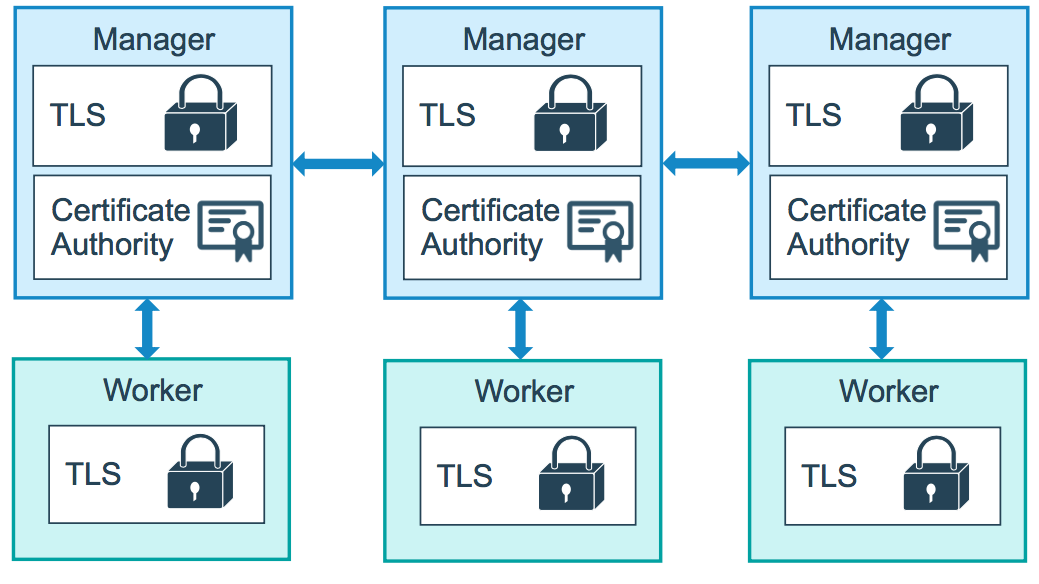
\includegraphics[width=.5\textwidth]{images/swarm-mode-pki.png}
  \caption{This figure illustrates how worker manager nodes and worker nodes 
encrypt communications using TLS
  \label{fig-swarm-pki} }
\end{figure}

The example below shows the information from a certificate from a worker
node:

\begin{quote}
Certificate:
    Data:
        Version: 3 (0x2)
        Serial Number:
            3b:1c:06:91:73:fb:16:ff:69:c3:f7:a2:fe:96:c1:73:e2:80:97:3b
        Signature Algorithm: ecdsa-with-SHA256
        Issuer: CN=swarm-ca
        Validity
            Not Before: Aug 30 02:39:00 2016 GMT
            Not After : Nov 28 03:39:00 2016 GMT
        Subject: O=ec2adilxf4ngv7ev8fwsi61i7, OU=swarm-worker,
CN=dw02poa4vqvzxi5c10gm4pq2g
...snip...
\end{quote}

By default, each node in the swarm renews its certificate every three
months. You can run docker swarm update --cert-expiry <TIME PERIOD> to
configure the frequency for nodes to renew their certificates. The minimum
rotation value is 1 hour. Refer to the docker swarm update CLI reference.


 



...




\section{Evaluation}
\label{sec-evaluation}

\cappos{This part of the eval focuses on an empirical evaluation of the 
performance, overhead, latency, etc. of different operations described in the
paper.  The purpose is to show the reader that the system actually works
efficiently at scale.}
 
...

\begin{figure}[t]
  \center{}
  
\includegraphics[scale=.5]{images/FakeTimeEval}
  \caption{\emph{I like to sometimes create figures with fake data so that I 
think through what I want to show before running an experiment that takes 
days.  DEFINITELY LABEL THIS CLEARLY SO IT IS NEVER SUBMITTED.  Look how 
clearly I labeled this as fake data!!!}
  \label{fig-time-eval} }
\end{figure}

\section{Experiences With \sysname}
\label{SEC:experiences}

\cappos{This part of the eval focuses on little tweaks you learned from trying
the things in this work out in practice.  This is where you explain things that
are more 'hacks'.  For example, originally we thought we might need to have
a distributed server that tracked XYZ, but in the end, we found that just
setting up a server with a simple fail over seems to work well in practice...}

...


\section{Related Work}
\label{SEC:related-work}

\cappos{Explain the rough grouping of the related work at a high level}

\cappos{break it down into categories either by paragraph or so, or have subsections.}

\cappos{Be sure to mention enough about Vault and the Kubernetes Kerberos 
secrets efforts.  Ideally we'd compare against them in the eval, but this may
not be practical...}

\section{Conclusion}
\label{SEC:conclusion}
\cappos{Explain the few key takeaways.  Benefits, eval results, usage, what is 
new.  If code / data is available, reiterate.  optionally, explain future 
work.}






%\dmyyyydate
{\footnotesize \bibliographystyle{abbrv}
\bibliography{bibdata}}
% \theendnotes

\end{document}
